\chapter{Ergebnisse}\label{sec:ergebnisse}








Zur Lösung der in~\autoref{sec:modell} hergeleiteten Selbstkonsistenzgleichungen~\eqref{eq:gap_eq_half_filling_integral} bzw.~\eqref{eq:gap_eq_arbitrary_filling_integral}, wird eine Kombination aus Fixpunktiteration und Newtonverfahren verwendet.
Die dafür erforderliche Zustandsdichte $\rho(\epsilon)$ wird ebenfalls numerisch über die in Ref.~\cite{hanisch_lattice_1997} hergeleitete Formel berechnet (siehe~Abbildung~\ref{fig:DOS}).
Für die numerische Berechnung wird das Python-Paket \textit{scipy}~\cite{virtanen_scipy_2020} verwendet. 
Plots werden mit \textit{matplotlib}~\cite{hunter_matplotlib_2007} erstellt.

\begin{figure}[htbp]
    \centering
    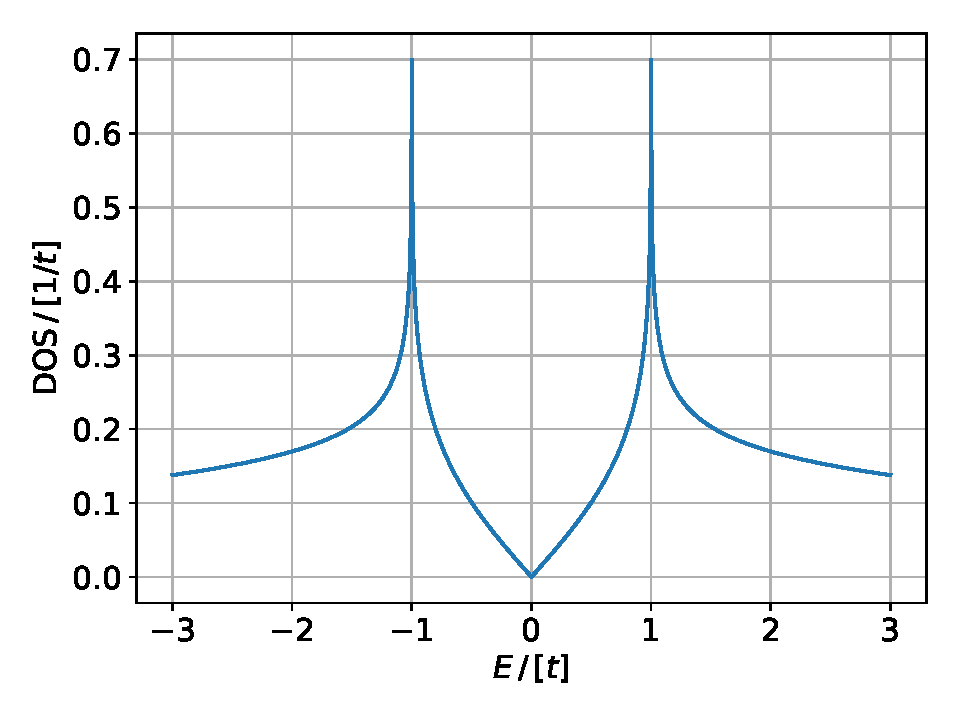
\includegraphics[width=0.7\textwidth]{Plots/DOS_complete.pdf}
    \caption{Zustandsdichte $\rho(E)$ (oder DOS  für engl. \textit{Density of States}) des Bienenwabengitters, berechnet nach der Formel in Ref.~\cite{hanisch_lattice_1997}. Energie $E$ ist in Einheiten des Hoppingparameters $t$ angegeben, die DOS  damit in Einheiten von $t^{-1}$. Die DOS  ist symmetrisch um $E=0$ und hat eine Van-Hove-Singularität (VHS) bei $E = \pm t$. Die Bandbreite $W$ beträgt $6t$ und die DOS verschwindet an den Dirac-Punkten ($E=0$).}
    \label{fig:DOS}
\end{figure}




















\section{Parameterabhängigkeiten von Ordnungsparameter und kritischer Temperatur}\label{sec:allgemein}

Es werden zunächst die allgemeinen Abhängigkeiten der kritischen Temperatur $T_C$ bzw. des Ordnungsparameters $\Delta$ von den Parametern Temperatur $T$, Wechselwirkungsstärke $U$, Debye-Energie $E_D = \hbar \omega_D$ und chemischem Potential $\mu$ geklärt.

Abbildung~\ref{fig:delta_vs_TndU} zeigt mit dem Plot links, dass $\Delta$ wie erwartet oberhalb einer kritischen Temperatur $T_C$ verschwindet und einen für die BCS-Theorie aufgrund der Mean-Field-Näherung typischen Kurvenverlauf, bestehend aus exponentiellem Plateau und Wurzelverhalten in der Nähe von $T_C$, aufweist~\cite{bardeen_theory_1957,tinkham_introduction_2004,czycholl_theoretische_2017}. 
Ebenfalls ist erkenntlich, dass das eine endliche Verschiebung des chemischen Potentials $\mu$ die kritische Temperatur $T_C$ im Vergleich zum undotierten Fall $\mu = 0$ deutlich erhöhen kann. 
Der Plot rechts zeigt, dass im dotierten Regime bereits eine minimale Wechselwirkung $U$ ausreicht, damit ein Ordnungsparameter $\Delta_0 \coloneqq \Delta(T=0)$ ausgebildet wird. 
Für $U \rightarrow 0$ geht $\Delta_0$ exponentiell fallend gegen Null, während erkennbar ist, dass $\Delta_0$ im undotierten Fall tatsächlich erst oberhalb einer kritischen Kopplung $U_C$ von null verschieden wird.


\begin{figure}[htb]
    \centering
    \begin{subfigure}{0.49\textwidth}
        \centering
        % \caption{}
        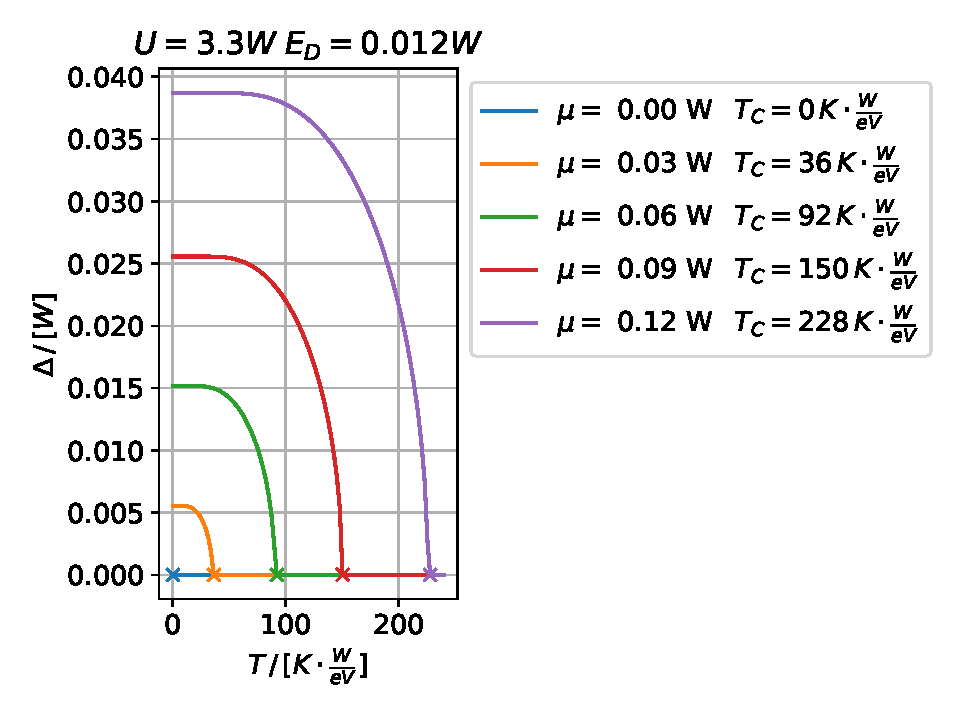
\includegraphics[width=\textwidth]{Plots/Delta_vs_T&mu_1.pdf}
        % \label{fig:delta_vs_t_mu}
    \end{subfigure}
    \hfill
    \begin{subfigure}{0.49\textwidth}
        \centering
        % \caption{}
        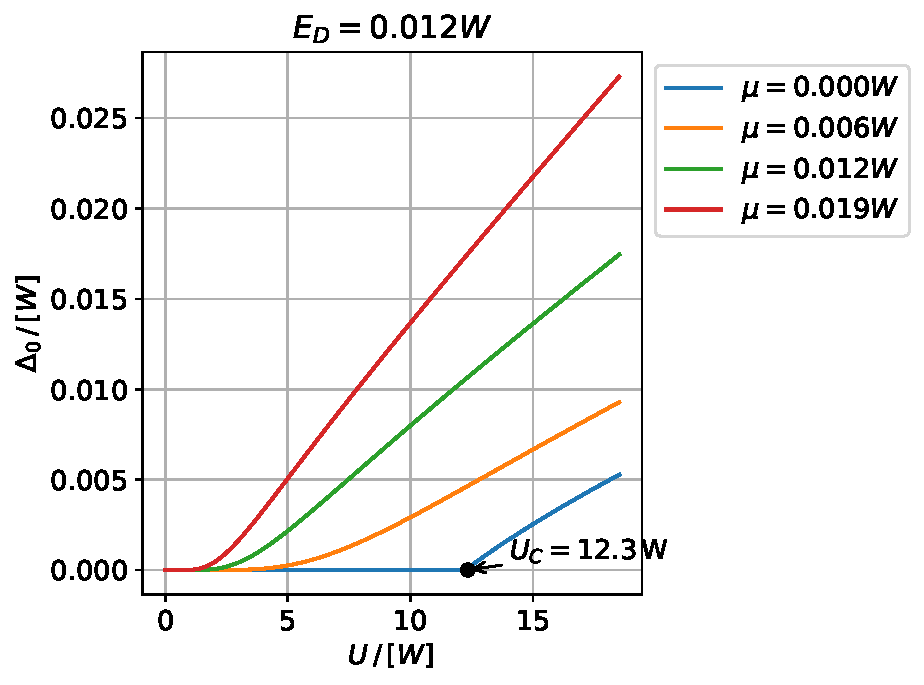
\includegraphics[width=\textwidth]{Plots/Delta_vs_U&mu_0.pdf}
        % \label{fig:delta_vs_u_mu}
    \end{subfigure}
    \caption{Abhängigkeiten des Ordnungsparameters $\Delta$ für verschiedene Dotierungsstärken $\mu$ in Einheiten der Bandbreite $W$. Links in Abhängigkeit von der Temperatur $T$ bei festen Parametern $U = \qty{3.3}{W}$ und $E_D = \qty{12e-3}{W}$ und rechts für verschiedene Kopplungsstärken $U$ bei $T= 0$ und $E_D = \qty{12e-3}{W}$ . Der Ordnungsparameter verschwindet oberhalb einer kritischen Temperatur $T_C$, die stark von $\mu$ abhängig ist und geht bei endlichem $\mu$ für kleine $U$ exponentiell fallend gegen null. Für $\mu = 0$ bildet sich ein endliches $\Delta_0$ erst oberhalb der kritischen Kopplung $U_C = \qty{12.3}{W}$  aus.}
    \label{fig:delta_vs_TndU}
\end{figure}

\subsection{Der quantenkritische Punkt bei halber Füllung}
Das Auftreten der kritischen Kopplungsstärke $U_C$ im Fall halber Füllung wurde ebenfalls in den Refs.~\cite{kopnin_bcs_2008,uchoa_superconducting_2007} bestätigt und dort als \glqq quantenkritischer Punkt\grqq{} bezeichnet.
Um diesen kritischen Punkt analytisch genauer zu untersuchen, wird die Selbstkonsistenzgleichung bei halber Füllung~\eqref{eq:gap_eq_half_filling_integral} für $\Delta \neq 0$ und $T = 0$ betrachtet:

\begin{align}
    1 = \frac{U}{2} \int_{-E_D}^{E_D} \frac{\rho(\epsilon)}{\sqrt{\epsilon^2 + \Delta_0^2}} \, d\epsilon~\label{eq:U_C_berechnen}
\end{align}

Da sich das Integral über die DOS im Allgemeinen nicht analytisch lösen lässt, bedarf es hier einer geeigneten Näherung. 
Klassischerweise wird die DOS oft einfach mit der Begründung, dass sie sich über das Intervall $[-E_D , E_D]$ kaum ändert als konstant $\rho(\epsilon) \approx \rho(E_F) = \rho(0)$ angenommen.
Diese Näherung führt genau zu dem exponentiell fallendem Verhalten, das in~Abbildung~\ref{fig:delta_vs_TndU} abseits von halber Füllung beobachtet wird~\cite{czycholl_theoretische_2017}.
Da die DOS aber bei halber Füllung am Energienullpunkt verschwindet, kann diese Näherung hier nicht durchgeführt werden. 
% Dies stellt allerdings kein Problem dar, denn die Näherung wäre wie bereits erwähnt zur Beschreibung der kritischen Kopplung auch nicht ausreichend.
Dies stellt allerdings kein Problem dar, da die konstante Näherung der DOS zur Beschreibung einer kritischen Kopplung ohnehin nicht ausreichen würde.

\begin{figure}
    \centering
    
\includegraphics[width=0.48\textwidth]{Plots/DOS.pdf}
    \caption{Vergleich der DOS  des Bienenwabengitters mit einer linearen Regression im Bereich $[-E_D, E_D]$ für $E_D = \qty{0.02}{W}$. Die lineare Regression liefert $A \approx \qty{6.6447}{W^{-2}}$.}
    \label{fig:DOS_regress}
\end{figure}

Stattdessen wird aufgrund der besonderen Form der DOS am Dirac-Punkt, die Näherung $\rho(\epsilon) \approx A \cdot \abs{\epsilon}$ verwendet, die für $E_D \ll W$ eine gute Übereinstimmung liefert (siehe~Abbildung~\ref{fig:DOS_regress}).
Für die meisten Festkörper ist die Bedingung $E_D \ll W$ bzw. $E_D/W \ll 1$ gut erfüllt, dennoch sollte diese bei einer konkreten Behandlung eines Materials konkret überprüft werden.
Die lineare Regression liefert die Steigung $A \approx \qty{6.6447}{W^{-2}}$.
Die Genaugkeit dieses Werts hängt jedoch ebenfalls von dem Verhältnis $E_D/W$ ab und ist hier für $E_D/W = 0.02$ berechnet worden.
% Die Genauigkeit dieser Näherung aber sicherlich von $E_D$ abhängt.
Eingesetzt in das Integral~\eqref{eq:U_C_berechnen} ergibt sich 
\begin{align}
    1 &= \frac{UA}{2} \int_{-E_D}^{E_D} \frac{\abs{\epsilon}}{\sqrt{\epsilon^2 + \Delta_0^2}} \, d\epsilon = UA \int_{0}^{E_D} \frac{\epsilon}{\sqrt{\epsilon^2 + \Delta_0^2}} \, d\epsilon = UA\left(\sqrt{E_D^2 + \Delta_0^2} - \Delta_0\right) \\
    &\implies U(\Delta_0) = \frac{1}{A\left(\sqrt{E_D^2 + \Delta_0^2} - \Delta_0\right)}~\label{eq:U_C}
\end{align}
und mit $U_C = \lim_{\Delta_0 \rightarrow 0} U(\Delta_0)$ erhält man $U_C = 1/(AE_D)$. 
Für $\mu \neq 0$ verschwindet die kritische Kopplung, was für $\abs{\mu} \gg E_D$ klar ist, da die DOS  dort sehr groß ist und die Näherung $\rho(\epsilon) \approx \rho(\mu)$ dort wieder gut geeignet ist~\cite{czycholl_theoretische_2017}.
Für eine schwache Ferminiveauverschiebung $\mu \sim E_D$ ist dies nicht so offensichtlich, im Anhang~\ref{sec:anhang_b} kann aber anhand der linearen Näherung der DOS gezeigt werden, dass für jedes $\mu \neq 0$ eine logarithmische Divergenz auftritt, sodass die kritische Kopplung verschwindet.
Es reicht also nicht, dass die DOS an der Fermi-Energie klein ist, sondern das Verschwinden von $\rho(\mu)$ ist ausschlaggebend für die Ausbildung des quantenkritischen Punkts.




















\subsection{Abhängigkeit von den Parametern \texorpdfstring{$U$, $E_D$ und $\mu$}{U, E_D und mu}}

Die Teilabbildung (a) aus Abbildung~\ref{fig:ALLG_ABH} zeigt bei halber Füllung, dass der zuvor hergeleitete hyperbolische Verlauf von $U_C$~\eqref{eq:U_C} gut von der Numerik bestätigt wird. 
Für kleine Debye-Energien $E_D$ ist also eine sehr große Kopplung nötig, während für große $E_D$ nur eine geringe Kopplung vonnöten ist, um ein endliches $\Delta_0$ auszubilden.
In Teilabbildung (b) ist der leicht dotierte Fall ($\mu = 0.02W$) zu sehen, der nun keine kritische Kopplung mehr aufweist. 
Er unterscheidet sich nicht sonderlich von Fall (a), da die Ordnungsparameter mit $U<U_C$ zwar endlich, aber dennoch klein sind, was in dieser Grafik nicht aufgelöst werden kann.
Die Teilabbildungen (c) und (d) zeigen für $\Delta_0$ und $T_C$ ähnliche Abhängigkeiten, was auf eine näherungsweise Proportionalität schließen lässt, wie in der BCS-Theorie mit dem universellen Verhältnis $2\Delta_0/(k_B T_C) = \num{3.53}$ erwartet wird~\cite{czycholl_theoretische_2017}.
Des Weiteren lässt sich erkennen, dass $\Delta_0$ im Bereich $\abs{\mu} < 0.05 \, W$ wie zu erwarten war stark unterdrückt wird, außerhalb davon aber stark mit dem chemischen Potential anwächst.
Sein Maximum befindet sich bei den Van-Hove-Singularitäten (VHS) bei $\mu = \pm t = \pm W/6$, wo sogar für $U< 1W$ in den Plots noch endliche $\Delta_0$ erkennbar sind.

\begin{figure}[htb]
    \centering
    \begin{subfigure}{0.38\textwidth}
        \centering
        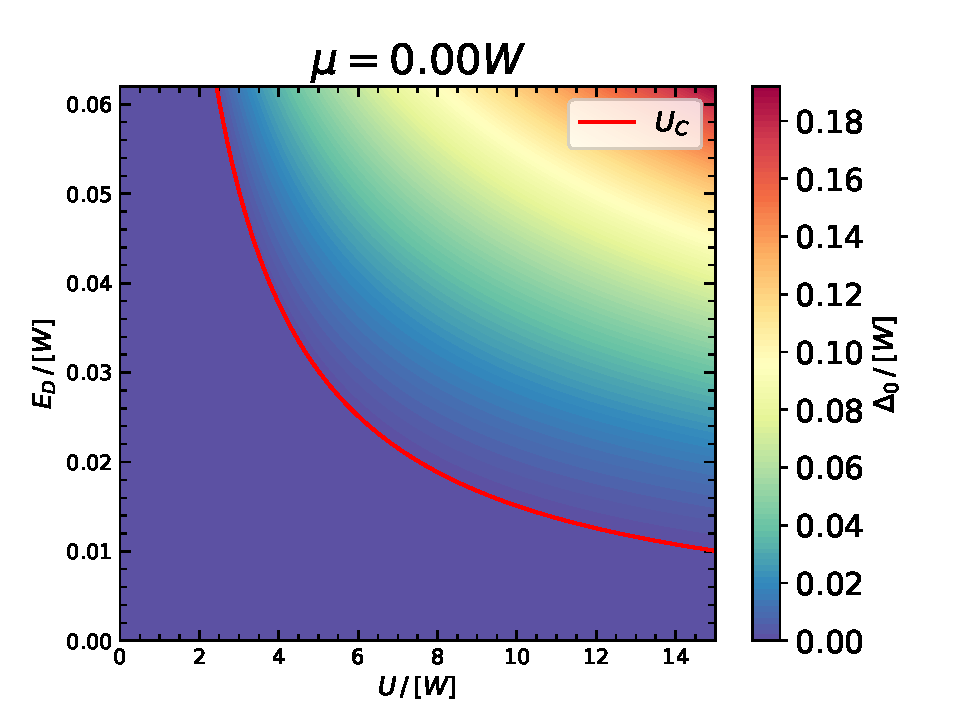
\includegraphics[width=\textwidth]{Plots/DELTA0_vs_E_D&U_0.pdf}
        \caption{}
    \end{subfigure}
    % \hfill
    \begin{subfigure}{0.38\textwidth}
        \centering
        
\includegraphics[width=\textwidth]{Plots/DELTA0_vs_E_D&U_1.pdf}
        \caption{}
    \end{subfigure}
    \vspace{-0.2cm}
    \begin{subfigure}{0.38\textwidth}
        \centering
        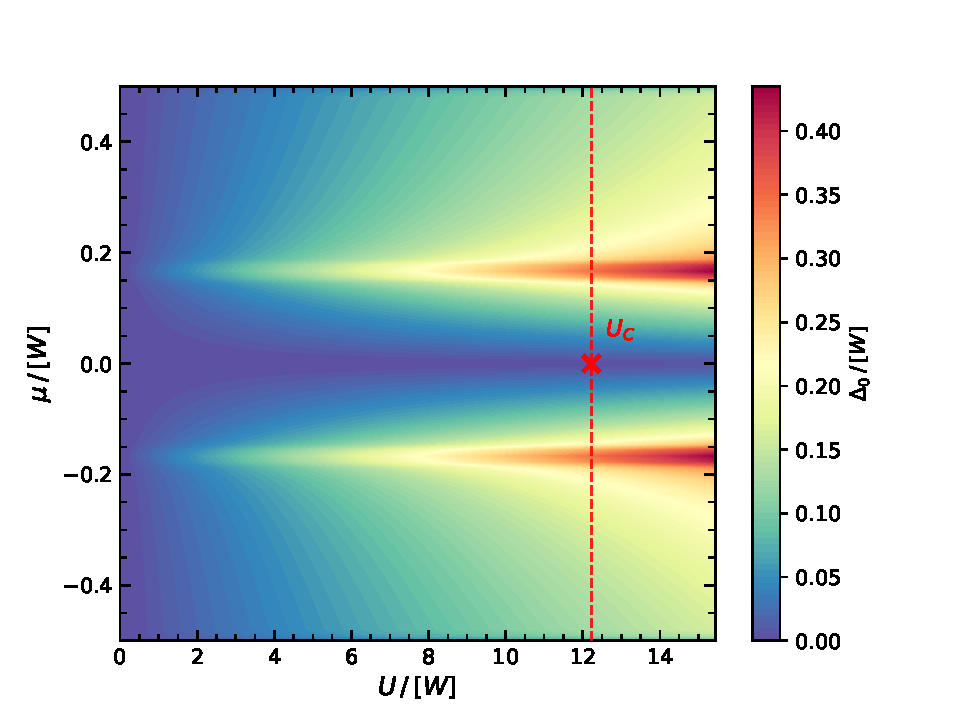
\includegraphics[width=\textwidth]{Plots/DELTA0_vs_mu&U_1.pdf}
        \caption{}
    \end{subfigure}
    % \hfill
    \begin{subfigure}{0.38\textwidth}
        \centering
        
\includegraphics[width=\textwidth]{Plots/TC_vs_mu&U_6.pdf}
        \caption{}
    \end{subfigure}
    \caption{
        (a) und (b) zeigen die Abhängigkeit des Ordnungsparameters $\Delta_0$ von Kopplung $U$ und Debye-Energie $E_D$, einmal für $\mu=0$ (a) und einmal für $\mu = \qty{0.02}{W}$ (b).
        (c) und (d) vergleichen bei $E_D = \qty{12e-3}{W}$ die Abhängigkeiten von $U$ und $\mu$ von $\Delta_0$ (c) und kritischer Temperatur $T_C$ (d). Die kritische Temperatur wird über die Selbstkonsistenzgleichung bei endlicher Temperatur berechnet.  In allen Teilabbildungen wird für die kritische Kopplung $U_C$ für $\mu = 0$ eingezeichnet.
    }
    \label{fig:ALLG_ABH}
\end{figure}



























\section{Konventionelle Supraleitung in Graphen}\label{sec:graphen}

Nachdem in Abschnitt~\ref{sec:allgemein} zunächst nur allgemeine Aussagen über die Abängigkeiten der für Supraleitung relevanten Größen getroffen wurden, wird nun konkret Graphen betrachtet um zu prüfen, ob realistische Bedingungen für $s$-wave Supraleitung erreichbar sind.
Andere Materialien mit Bienenwabengitter, wie das eingangs erwähnte $\mathrm{MoS_2}$, eignen sich für eine analoge Betrachtung dagegen nicht ohne Weiteres:
Andere Materialien mit Bienenwabengitter, wie das eingangs erwähnte $\mathrm{MoS_2}$, eignen sich für eine analoge Betrachtung dagegen nicht ohne Weiteres:
Zwar lassen sich mit $W \approx 12 - \qty{18}{eV}$~\cite{shahriari_band_2018} und einer Debye-Temperatur von $\Theta_D \approx \qty{262.3}{K}$~\cite{peng_thermal_2016} (entsprechend $E_D \approx \qty{22.6}{meV}$) konkrete Parameter zur Berechnung der supraleitenden Lücke angeben, allerdings sind die beiden Untergitter in $\mathrm{MoS_2}$ durch unterschiedliche Atome (Mo bzw.\ S) besetzt und mehrere Atomorbitale tragen zur elektronischen Struktur bei, sodass erst Tight-Binding-Modelle mit bis zu elf Bändern~\cite{jalilvand_multi-band_2020, shahriari_band_2018} eine ausreichend genaue Beschreibung liefern.
So ergibt sich für $\mathrm{MoS_2}$ beispielsweise statt eines Dirac-Punktes eine endliche Bandlücke.
Das in dieser Arbeit verwendete Ein-Orbital-Modell kann diese Eigenschaft prinzipiell nicht abbilden und wird im Folgenden daher nur auf Graphen angewendet.

Für Graphen wird üblicherweise ein Hüpfparameter von $t=\qty{2.7}{eV}$ gewählt, der die $\pi$- und $\pi^*$-Bänder beschreibt~\cite{castro_neto_electronic_2009, kundu_tight_2009,peres_colloquium_2010}.
Damit ergibt sich eine Bandbreite von $W = 6 t = \qty{16.2}{eV}$, während die Debye-Temperatur von Graphen je nach Mode im Bereich von $\Theta_D = \num{1287} - \qty{2300}K$ liegt~\cite{tewary_singular_2009}.
Das entspricht einer Debye-Energie von $E_D \approx \num{110} - \qty{198}{meV}$, wobei hier als Best-Case-Abschätzung $E_D \approx \qty{200}{\milli\electronvolt}$ gewählt wird.
Das Verhältnis zwischen Debye-Energie und Bandbreite ergibt sich damit zu $E_D/W \approx \num{12.33e-3}$, was sogar noch unter dem in Abbildung~\ref{fig:DOS_regress} gewählten Verhältnis liegt, wofür die lineare Regression bereits ausgezeichnet war. 

Die Kopplungsstärke $U$ ist in der BCS-Theorie ein phänomenologischer Modellparameter, d.h.\ sie wird quantitativ nicht über die zugrundeliegende Elektron-Phonon-Wechselwirkung bestimmt sondern meist aus experimentellen Daten gefittet, sodass die Lücke $\Delta$ der BCS-Rechnung und des Experiments übereinstimmen. 
Tatsächliche \textit{ab initio} Rechnungen sind prinzipiell möglich, siehe dazu z.B.\ Refs.~\cite{giustino_electron-phonon_2017,morel_calculation_1962}, gehen aber weit über die BCS-Theorie hinaus und werden hier dementsprechend nicht betrachtet.
Für konventionelle Supraleiter kann $U$ anhand von $U = -1/\left(\ln\left(\sfrac{\Delta_0}{2E_D}\right)\rho_0\right) $~\cite{czycholl_theoretische_2017} grob abgeschätzt werden.
Die Bandlücke $\Delta$ liegt für die meisten konventionellen Supraleiter im einstelligen $\mathrm{meV}$-Bereich~\cite{croitoru_phonon_2015,czycholl_theoretische_2016}, für Niob beispielsweise ergibt sich mit $\Delta_0 = \qty{1.43}{\milli\electronvolt}$, $E_D = \qty{23}{meV}$~\cite{zarea_effects_2023} und $\rho_0 \approx \qty{2.07}{\per\electronvolt}$~\cite{anderson_self-consistent_1973} ein $U \approx \qty{0.14}{eV}$.
Es ist zu erwarten, dass $U$ in Graphen nicht um mehrere Größenordnungen von diesem Wert abweicht, für genauere Abschätzungen sind allerdings experimentelle Daten vonnöten.
Zum Beispiel liefern Herrera et al.\ \cite{herrera_topological_2024} explizite Vorhersagen für die kritische Temperatur in stark $\mathrm{Tb}$-dotiertem Graphen.
Sie sagen bei einer Dotierung bis zur VHS, eine kritische Temperatur von bis zu $T_C = \qty{600}{\milli\kelvin}$ voraus.
In diesem Tight-Binding Modell entspräche dies einem chemischen Potential von $\mu = t = \qty{2.7}{eV}$, Herrera et al.\ berichten allerdings nur von einer Ferminiveauverschiebung um $\qty{1.55}{eV}$ bei gleichzeitigem Abflachen der Energiebänder und Vergrößerung der VHS.
Diese Effekte werden in dem Modell in dieser Arbeit nicht behandelt, ein Vergleich im nächsten Abschnitt ist unter Vorbehalt allerdings trotzdem möglich.



















\subsection{Realistische Bedingungen für Supraleitung in Graphen}\label{sec:graphen_dotierung}

Es soll zum einen überprüft werden, wie stark die Kopplung in Graphen sein müsste, damit bei halber Füllung bzw.\ schwacher Dotierung eine supraleitende Bandlücke entsteht. 
Zum anderen soll eine Aussage darüber getätigt werden, für welche Dotierungsstärke $\mu$ innerhalb des abgeschätzten Bereichs von $U$ mit besonderem Augenmerk auf die VHS, Supraleitung zu erwarten ist.


\begin{figure}[htb]
    \centering
    \begin{subfigure}{0.48\textwidth}
        \centering
        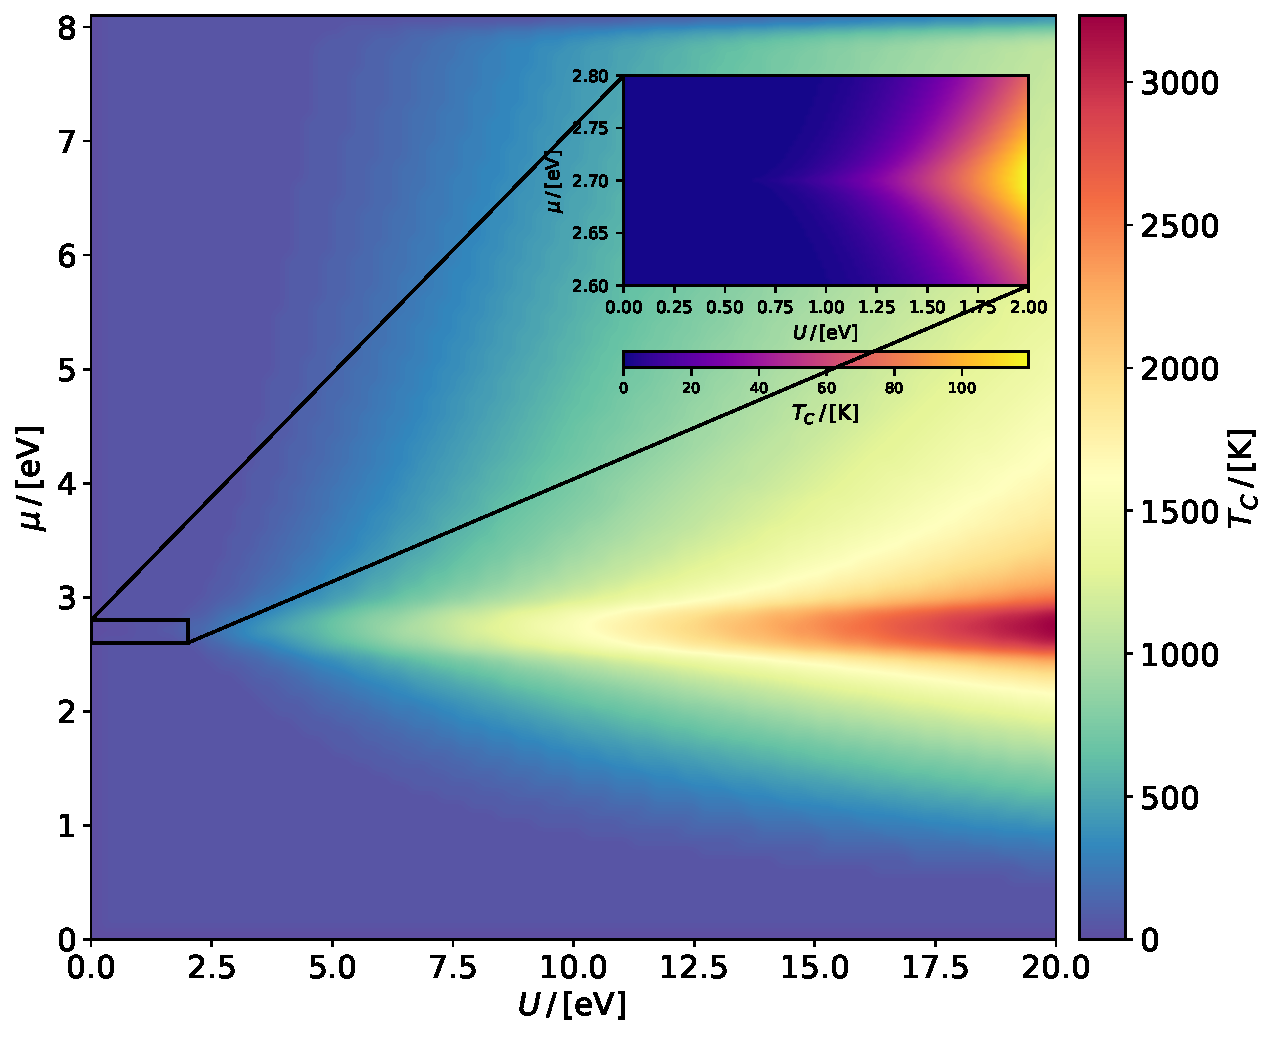
\includegraphics[width=\textwidth]{Plots/Plot_zusammen2.pdf}
        \caption{}
    \end{subfigure}
    \hfill
    \begin{subfigure}{0.48\textwidth}
        \centering
        
\includegraphics[width=\textwidth]{Plots/Plot_zusammen4.pdf}
        \caption{}
    \end{subfigure}
    \\
    \begin{subfigure}{0.48\textwidth}
        \centering
        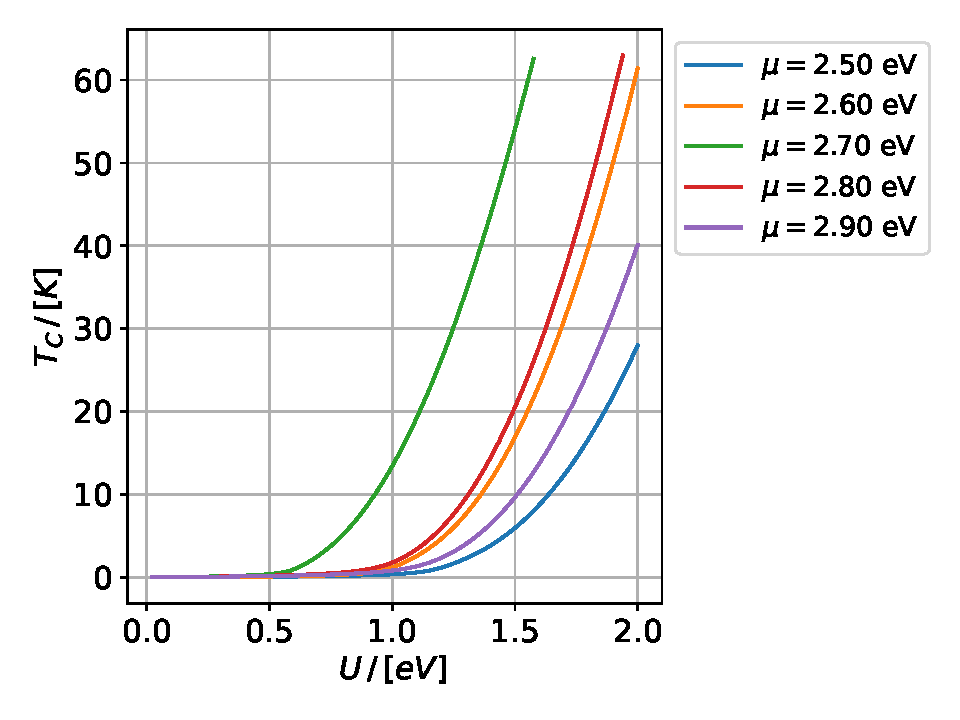
\includegraphics[width=\textwidth]{Plots/TC_vs_mu&U_fine_8.pdf}
        \caption{}
    \end{subfigure}
    \hfill
    \begin{subfigure}{0.48\textwidth}
        \centering
        
\includegraphics[width=\textwidth]{Plots/TC_vs_mu&U_fine_7.pdf}
        \caption{}
    \end{subfigure}
    \caption{Kritische Temperatur $T_C$ in Abhängigkeit von Kopplung $U$ und chemischem Potential $\mu$. In Teilabbildung (a) ist eine Detailansicht des Bereichs um die VHS dargestellt und in (b) um den Bereich des quantenkritischen Punkts. In (c) und (d) ist der Gesamtverlauf um die VHS herum zu sehen, wobei (d) eine Vergrößerung auf den Bereich bis maximal $T_C = \qty{1}{K}$ darstellt.}
    \label{fig:TC_Graphen}
\end{figure}

% In Abbildung~\ref{fig:TC_Graphen} ist dargestellt, wie sich $T_C$ als Funktion von $U$ und $\mu$ ändert. 
% Die Teilabbildung (a) zeigt zusätzlich eine Detailansicht des Bereichs um die VHS, während Teilabbildung (b) den Bereich um den quantenkritischen Punkt bei $\mu = 0$ genauer darstellt.
Abbildung~\ref{fig:TC_Graphen} zeigt die kritische Temperatur $T_C$ in Abhängigkeit von $U$ und $\mu$. 
Teilabbildung (a) stellt den Gesamtverlauf um die VHS dar, mit einer Detailansicht des unmittelbaren VHS-Bereichs, während Teilabbildung (b) entsprechend den Gesamtverlauf mit einer Detailansicht um den quantenkritischen Punkt bei $\mu = 0$ zeigt.
In den Teilabbildungen (c) und (d) sind jeweils Schnitte $T_C(U)$ für feste $\mu$ um die VHS herum zu sehen, wobei in (d) eine Vergrößerung auf den Bereich bis maximal $T_C = \qty{1}{K}$ zu sehen ist.

Es ist zu erkennen, dass an der VHS bei Kopplungen in der für konventionelle Supraleiter typischen Größenordnung von ca. $\qty{0.1}{eV}$ verhältnismäßig große kritische Temperaturen auftreten, während dies bei halber Füllung erst ab einer kritischen Kopplung von $U_C \approx \qty{198}{eV}$ der Fall ist, was deutlich über dem realistischen Bereich von $U$ liegt.
Damit kann konventionelle Supraleitung im undotierten Fall ausgeschlossen werden.

Der Vergleich mit Ref.~\cite{herrera_topological_2024} zeigt, dass die dort vorhergesagte kritische Temperatur $T_C = \qty{600}{\milli\kelvin}$, hier für $U$ in dem Bereich $\num{0.5} - \qty{1.1}{eV}$ reproduziert wird (siehe Teilabbildungen (c) und (d)).
Dieser Wert liegt über dem für Niob abgeschätzten Wert, allerdings in einer vergleichbaren Größenordnung und ist damit nicht unbedingt unrealistisch. 
Anhand dieser Abschätzung ist also nicht auszuschließen, dass (stark) dotiertes Graphen konventionelle Supraleitung zeigen kann.
Diese Beobachtung ist ebenfalls durch Ludbrook et al.\ \cite{ludbrook_evidence_2015} gestützt, die in Li-dotiertem Graphen bei $T = \qty{3.5}{K}$ eine Bandlücke von $\Delta = \qty{0.9}{meV}$ experimentell bestätigen konnten.
Hierbei wäre ein ebenfalls eine genauerer Vergleich mit einem direkten Wert des chemischen Potentials $\mu$ interessant, das allerdings nicht direkt angegeben wurde.